% mainfile: ../../main.tex
\setchapterpreamble[u]{\margintoc}
\chapter{Supplementary to Part \ref{part:ff}: Filter-function derivations and validation}\label{ch:app:ff}
In this appendix, we give additional information on the filter-function formalism presented in \cref{part:ff}.
We first show additional derivations that were omitted from the main text in \cref{sec:app:ff:derivations}, and derive bounds on the \gls{me} convergence in  \cref{sec:app:ff:convergence}.
In \cref{sec:app:ff:concatenation}, we augment the \gls{ff} formalism of the main text by deriving a concatenation rule for the second-order terms of the \gls{me}.
This enables a more efficient calculation of the full quantum process including coherent errors for sequences of quantum gates together with the rule for first-order terms given in \cref{subsec:ff:theory:control_matrix:sequence}.
In \cref{sec:app:ff:time_domain_methods}, we review time-domain simulation methods of noisy quantum dynamics, which we employ in \cref{sec:app:ff:fidelity} to validate our \gls{ff} formalism's predicted fidelities for the quantum gates of \citer{Cerfontaine2020} and discussed in \cref{sec:ff:examples:optimized_gates}, as well as the \gls{qft} algorithm presented in \cref{sec:ff:examples:qft}.
We use the notation set in \cref{sec:ff:theory:transfer_matrix} except where indicated otherwise.

% ==================================================
%           DERIVATION SECTION
% ==================================================
\section{Additional derivations}\label{sec:app:ff:derivations}
\subsection{Derivation of the single-qubit cumulant function in the Liouville representation}\label{subsec:app:ff:derivations:cumulant:pauli}
For a single qubit, the Pauli basis $\mc{P}_1 = \left\lbrace\sigma_i\right\rbrace_{i=0}^3 = 1/\sqrt{2}\times\left\lbrace\eye,\sx,\sy,\sz\right\rbrace$ is a natural choice to define the Liouville representation.
In this case, the trace tensor \cref{eq:ff:trace_tensor} can be simplified and thus \cref{eq:ff:cumulant:truncated:liouville} given a more intuitive form which we derive in this subsection.
Since the cumulant function is linear in the noise indices $\alpha,\beta$ we drop them in the following for legibility.
Our results hold for both a single pair of noise indices and the total cumulant.
We start by observing the relation
\begin{equation}\label{eq:ff:trace_tensor:four_paulis}
    T_{klij} = \tr(\sigma_k\sigma_l\sigma_i\sigma_j) = \frac{1}{2}(\delta_{kl}\delta_{ij} - \delta_{ki}\delta_{lj} + \delta_{kj}\delta_{li})
\end{equation}
for the Pauli basis elements $\sigma_k, k\in\lbrace 1, 2, 3\rbrace$.
Including the identity element $\sigma_0$ in the trace tensor gives additional terms.
However, as we show now none of these contribute to \cumulantfun because they cancel out.

First, since the noise Hamiltonian $\Hn(t)$ is traceless and therefore $\ctrlmat_{\alpha 0}(t) = 0$, we have $\decayamps_{kl},\freqshifts_{kl}\propto (1 - \delta_{k0})(1 - \delta_{0l})$, \ie the first column and row of both the decay amplitude and frequency shift matrices are zero, and hence terms in the sum of \cref{eq:ff:cumulant:truncated:liouville} with either $k = 0$ or $l = 0$ vanish.
Next, for $i = j = 0$ all of the traces cancel out as can be easily seen.
The last possible cases are given by $i = 0, j\neq 0$ and vice versa.
For these cases we have
\begin{equation}\label{eq:ff:trace_tensor:three_paulis}
    T_{kl0j} = T_{klj0} = \frac{1}{\sqrt{2}}\tr(\sigma_k\sigma_l\sigma_j) = \frac{\i}{2}\varepsilon_{klj}
\end{equation}
with $\varepsilon_{klj}$ the completely antisymmetric tensor.
Both of the above cases vanish in \cumulantfun since, taking the case $j = 0$ for example,
\begin{subequations}\label{eq:ff:trace_tensor:three_paulis:aggregate}
\begin{equation} \label{eq:ff:trace_tensor:three_paulis:aggregate:decayamps}
    \frac{1}{2}\left(T_{kl0i} - T_{k0li} - T_{kil0} + T_{ki0l}\right) =
    \frac{\i}{2}\left(\varepsilon_{kli} - \varepsilon_{kli} - \varepsilon_{kil} + \varepsilon_{kil}\right) = 0
\end{equation}
for the decay amplitudes \decayamps and
\begin{equation} \label{eq:ff:trace_tensor:three_paulis:aggregate:freqshifts}
    \frac{1}{2}\left(T_{kl0i} - T_{lk0i} - T_{kli0} + T_{lki0}\right) =
    \frac{\i}{2}\left(\varepsilon_{kli} - \varepsilon_{lki} - \varepsilon_{kli} + \varepsilon_{lki}\right) = 0
\end{equation}
\end{subequations}
for the frequency shifts \freqshifts.
Hence, only terms with $i,j > 0$ contribute and we can plug the simplified expressions for the trace tensor $T_{klij}$, \cref{eq:ff:trace_tensor:four_paulis}, into \cref{eq:ff:cumulant:truncated:liouville} to write the cumulant function for a single qubit and the Pauli basis concisely as
\begin{align}
    \cumulantfun_{ij}(\tau) &= -\frac{1}{2}\sum_{kl}\begin{aligned}[t]\Bigl[
                                   &\freqshifts_{kl}\left(T_{klji} - T_{lkji} - T_{klij} + T_{lkij}\right) \\
                                   &+ \decayamps_{kl}\left(T_{klji} - T_{kjli} - T_{kilj} + T_{kijl}\right)
                               \Bigr]\end{aligned} \\
                            &= -\sum_{kl}\left[\freqshifts_{kl}(\delta_{ki}\delta_{lj} - \delta_{kj}\delta_{li})
                                               + \decayamps_{kl}(\delta_{kl}\delta_{ij} - \delta_{kj}\delta_{li})\right] \\
                            &= \freqshifts_{ji} - \freqshifts_{ij} + \decayamps_{ij} - \delta_{ij}\tr\decayamps \\
                            &= \begin{dcases}
                                  - \sum_{k\neq i}\decayamps_{kk}                           &\qif* i = j,   \\
                                  - \freqshifts_{ij} + \freqshifts_{ji} + \decayamps_{ij}   &\qif* i\neq j,
                               \end{dcases}
\end{align}
as given in the main text.

\subsection{Evaluation of the integrals in \cref{eq:ff:frequency_shifts:freq}}\label{subsec:app:ff:derivations:frequency_shifts:integral}
Here we calculate the integrals appearing in the calculation of the frequency shifts \freqshifts, \cref{eq:ff:frequency_shifts:integral}, given by
\begin{equation}
    I_{ijmn}\gth{g}(\omega) = \int_{t_{g-1}}^{t_g}\dd{t}\e^{\i\Omega_{ij}\gth{g}(t - t_{g-1}) - \i\omega t}
                              \int_{t_{g-1}}^{t}\dd{t^\prime}\e^{\i\Omega_{mn}\gth{g}(t^\prime - t_{g-1}) + \i\omega t^\prime}.
\end{equation}
The inner integration is simple to perform and we get
\begin{multline}
    I_{ijmn}\gth{g}(\omega) = \int_{t_{g-1}}^{t_g}\dd{t}\e^{\i\Omega_{ij}\gth{g}(t - t_{g-1}) - \i\omega(t - t_{g-1})}\\
    \times\begin{dcases}
        \frac{\e^{\i(\omega + \Omega_{mn}\gth{g})(t - t_{g-1})} - 1}{\i(\omega + \Omega_{mn}\gth{g})}   &\qif* \omega + \Omega_{mn}\gth{g}\neq 0 \\
        t - t_{g-1}                                                                                     &\qif* \omega + \Omega_{mn}\gth{g} = 0.
    \end{dcases}
\end{multline}
Shifting the limits of integration and performing integration by parts in the case $\omega + \Omega_{mn}\gth{g} = 0$ then yields
\begin{align}
    &I_{ijmn}\gth{g}(\omega) = \\
    &\begin{cases}
        \frac{1}{\omega + \Omega_{mn}\gth{g}}\left(
            \frac{\e^{\i(\Omega_{ij}\gth{g} - \omega)\Delta t_g} - 1}{\Omega_{ij}\gth{g} - \omega} -
            \frac{\e^{\i(\Omega_{ij}\gth{g} + \Omega_{mn}\gth{g})\Delta t_g} - 1}{\Omega_{ij}\gth{g} + \Omega_{mn}\gth{g}}
        \right) &\text{if } \omega + \Omega_{mn}\gth{g}\neq 0, \\
        \frac{1}{\Omega_{ij}\gth{g} - \omega}\left(
            \frac{\e^{\i(\Omega_{ij}\gth{g} - \omega)\Delta t_g} - 1}{\Omega_{ij}\gth{g} - \omega} -
            \i\Delta t_g\e^{\i(\Omega_{ij}\gth{g} - \omega)\Delta t_g}
        \right) &\text{if } \omega + \Omega_{mn}\gth{g} = 0 \wedge \Omega_{ij}\gth{g} - \omega\neq 0, \\
        \frac{\Delta t_g^2}{2} &\text{if } \omega + \Omega_{mn}\gth{g} = 0 \wedge \Omega_{ij}\gth{g} - \omega = 0.
    \end{cases} \notag
\end{align}

\subsection{Simplifying the calculation of the entanglement infidelity}\label{subsec:app:ff:derivations:fidelity}
In the main text, we claimed that the contribution of noise sources $(\alpha,\beta)$ to the total entanglement infidelity $\entinfid(\liouvUe) = \sum_{\alpha\beta}\infid_{\alpha\beta}$ reduces from the trace of the cumulant function \cumulantfun to
\begin{align}
    \infid_{\alpha\beta} &= -\frac{1}{d^2}\tr\cumulantfun_{\alpha\beta} \label{eq:app:ff:infid} \\
                         &= \frac{1}{d}\tr\decayamps_{\alpha\beta}.
\end{align}
To show this, we substitute \cumulantfun by its definition in terms of \freqshifts and \decayamps according to \cref{eq:ff:cumulant:truncated:liouville}.
This yields for the trace
\begin{equation}\label{eq:app:ff:cumulant:trace:1}
    \begin{split}
        \tr\cumulantfun_{\alpha\beta} &= -\frac{1}{2}\sum_{kl}\delta_{ij}(f_{ijkl}\freqshifts_{\alpha\beta,kl} + g_{ijkl}\decayamps_{\alpha\beta,kl}) \\
                                      &= -\frac{1}{2}\sum_{ikl}\decayamps_{\alpha\beta,kl}\left(T_{klii} + T_{lkii} - 2 T_{kili}\right)
    \end{split}
\end{equation}
since \freqshifts is antisymmetric.
In order to further simplify the trace tensors on the right hand side of \cref{eq:app:ff:cumulant:trace:1}, we observe that the orthonormality and completeness of the operator basis \basis defining the Liouville representation of \cumulantfun (\cf \cref{eq:ff:basis}) is equivalent to requiring that $\basis\adjoint\basis = \eye$ with \basis reshaped into a $d^2\times d^2$ matrix by a suitable mapping.
This condition may also be written as
\begin{equation}\label{eq:ff:basis:identity}
\begin{split}
    \delta_{ac}\delta_{bd} &= \sum_{k} C^\ast_{k,ab} C_{k,cd} \\
                           &= \sum_{k} C_{k,ba} C_{k,cd}
\end{split}
\end{equation}
because every element $C_k$ is Hermitian.
Using this relation in \cref{eq:app:ff:cumulant:trace:1} then yields
\begin{equation}\label{eq:app:ff:cumulant:trace:2}
    \begin{split}
        \tr\cumulantfun_{\alpha\beta} &= -\frac{1}{2}\sum_{kl}\decayamps_{\alpha\beta,kl}\left(2d\delta_{kl} - 2\tr(C_k)\tr(C_l)\right) \\
                                      &= -d\tr\decayamps_{\alpha\beta}.
    \end{split}
\end{equation}
The last equality only holds true for bases with a single non-traceless element (the identity), such as the bases discussed in \cref{sec:ff:performance:basis}.
This is because in this case, $\tr(C_k) = 0$ for $k > 0$ whereas $\decayamps_{\alpha\beta,kl} = 0$ for either $k = 0$ or $l = 0$ since \decayamps is a function of the traceless noise Hamiltonian for which $\tr(C_0\Hn) \propto \tr\Hn = 0$ (\ie the first column of the control matrix is zero, see \cref{eq:ff:control_matrix,eq:ff:decay_amplitudes:time}).
Finally, substituting \cref{eq:app:ff:cumulant:trace:2} into \cref{eq:app:ff:infid} we obtain our result
\begin{equation}
    \infid_{\alpha\beta} = \frac{1}{d}\tr\decayamps_{\alpha\beta}.
\end{equation}

% ==================================================
%                  SUM RULE SECTION
% ==================================================
\subsection{Sum rule}\label{subsec:app:ff:sum_rule}
For white noise, the infidelity to leading order does not depend on the internal dynamics of the control operation but only on the total duration $\tau$.
To see this, take \cref{eq:ff:decay_amplitudes:time} and substitute the correlation function of white noise, $\ev{b_\alpha(t_1)b_\alpha(t_2)}=S_0\delta(t_1-t_2)$.
The integrals then simplify to
\begin{equation}
    \decayamps_{\alpha\alpha,kl} = S_0\int_0^{\tau}\dd{t}\ctrlmat_{\alpha k}(t)\ctrlmat_{\alpha l}(t).
\end{equation}
In order to compute the infidelity, we require the trace over the matrix of decay amplitudes (\cref{eq:ff:infidelity:ent}), so
\begin{equation}
    I_{\alpha} = \frac{S_0}{d}\trace\decayamps_{\alpha\alpha} = \frac{1}{d}\sum_k\int_0^{\tau}\dd{t}\ctrlmat_{\alpha k}^2(t).
\end{equation}
Now recall that \ctrlmat is a vector on Liouville space and we can write $\ctrlmat_{\alpha}(t)\doteq\dket*{\Bat(t)}\equiv\dbra*{\Bat(t)}$ because it is Hermitian.
Thus,
\begin{equation}
    I_{\alpha} = \frac{S_0}{d}\int_0^{\tau}\dd{t}\dip*{\Bat(t)}{\Bat(t)} = \frac{1}{d}\int_0^{\tau}\dd{t}\norm{\Bat(t)}^2,
\end{equation}
and if $\Ba(t)=\Ba$, \ie, is time-independent, the integral evaluates simply to $\tau$,
\begin{equation}
    I_{\alpha} = \frac{S_0\tau}{d}\norm{\Bat}^2,
\end{equation}
because the control unitary $\Uc(t)$ conserves the norm.
Since also $I_{\alpha}=\int\dd{\omega}/2\pi d\,S(\omega)\FF_\alpha(\omega)$ with the fidelity filter function $\FF_\alpha(\omega)$ (\cref{eq:ff:filter_function:fidelity,eq:ff:infidelity:ent:integral}), this result also implies the sum rule
\begin{equation}\label{eq:app:ff:sum_rule}
    \int\ddf{\omega}\FF_{\alpha}(\omega) = \tau\norm{\Bat}^2,
\end{equation}
a result previously obtained by \citet{Cywinski2008}.
This means that pulse shaping and similar techniques never yield a leading-order fidelity enhancement if the noise is white in the relevant regime of frequencies as the fidelity only depends on the total duration of the pulse.

% ==================================================
%           CONVERGENCE SECTION
% ==================================================
\section{Convergence Bounds}\label{sec:app:ff:convergence}
In this section we give bounds for the convergence of the expansions employed in the main text for the case of purely autocorrelated noise, $S_{\alpha\beta}(\omega) = \delta_{\alpha\beta}S_{\alpha\beta}(\omega) =  S_\alpha(\omega)$, following the approach by~\citet{Green2013}.
For Gaussian noise, our expansion is exact when including first and second order \acrfull{me} terms.
Hence, the convergence radius of the \gls{me} becomes infinite and the fidelity can be computed exactly by evaluating the matrix exponential \cref{eq:ff:cumulant}.
For non-Gaussian noise, the following considerations apply.
\subsection{Magnus Expansion}\label{subsec:app:ff:convergence:magnus_expansion}
The \gls{me} of the error propagator \cref{eq:ff:magnus_expansion:1} converges if $\int_0^\tau\dd{t}\norm*{\Hnt(t)} < \pi$ with $\norm{A}^2 = \dotHS{A}{A} = \sum_{ij}\lvert A_{ij}\rvert^2$ the Frobenius norm~\cite{Moan1999}.
We assume a time dependence of the noise operators of the form $\Ba(t) = s_\alpha(t)\Ba$.
By the Cauchy-Schwarz inequality we then have
\begin{equation}
    \begin{split}
        \bigl\lVert\Hnt(t)\bigr\rVert^2 &= \norm{\Hn(t)}^2 \\
                          &= \sum_{\alpha\beta} s_\alpha(t) s_{\beta}(t) b_\alpha(t) b_{\beta}(t)\dotHS{B_\alpha}{B_{\beta}} \\
                          &\leq\sum_{\alpha\beta} s_\alpha(t) s_{\beta}(t) b_\alpha(t) b_{\beta}(t)
                             \norm*{B_\alpha}\norm*{B_{\beta}} \\
                          &\leq\biggl[\sum_{\alpha}\sum_{g=1}^{G}\vartheta\gth{m}(t)
                             s_\alpha\gth{m}b_\alpha\gth{m}\norm{B_\alpha}\biggr]^2
    \end{split}
\end{equation}
where $b_{\alpha}\gth{m}$ is the maximum value that the noise assumes during the pulse, $\vartheta\gth{g}(t) = \theta(t - t_{g-1}) - \theta(t - t_g)$ is one during the $g$th time interval and zero else, and where we approximated the time evolution as piecewise constant.
Then, in order to guarantee convergence of the \gls{me},
\begin{equation}
    \begin{split}
        \int_0^{\tau}\dd{t}\norm*{\Hnt(t)} &\leq\int_0^\tau\dd{t}\abs\bigg{\sum_{\alpha}\sum_{g=1}^{G}
                                              \vartheta\gth{m}(t) s_\alpha\gth{m} b_\alpha\gth{m}\norm{B_\alpha}} \\
                                           &= \sum_{\alpha} b_\alpha\gth{m}\norm{B_\alpha}\sum_{g=1}^{G}s_\alpha\gth{m}
                                              \int_{t_{g-1}}^{t_{g}}\dd{t} \\
                                           &= \sum_{\alpha} C_m\delta b_\alpha\norm{B_\alpha}\sum_{g=1}^{G}
                                              s_\alpha\gth{m}\Delta t_g \\
                                           &\eqqcolon N
    \end{split}
\end{equation}
where we have expressed the in principle unknown maximum noise amplitude $b_\alpha\gth{m}$ in terms of the root mean square value $\delta b_\alpha$.
That is, $b_\alpha\gth{m} = C_m \expval*{b_\alpha(0)^2}^{1/2} =  C_m \delta b_\alpha$ for a sufficiently large value $C_m$.
Finally, realizing that $\delta b_\alpha^2 = \int\frac{\dd{\omega}}{2\pi} S_\alpha(\omega)$ and by the triangle inequality,
\begin{equation}
    \begin{split}
        N &= C_m\sum_{\alpha}\norm{B_\alpha}\biggl[\int_{-\infty}^\infty\frac{\mathrm{d}\omega}{2\pi} S_\alpha(\omega)\biggr]^{1/2}
            \sum_{g=1}^{G} s_\alpha\gth{m}\Delta t_g \\
          &\leq C_m\biggl[\sum_{\alpha}\norm{B_\alpha}^2\int_{-\infty}^\infty\frac{\mathrm{d}\omega}{2\pi} S_\alpha(\omega)
            \biggl(\sum_{g=1}^{G} s_\alpha\gth{m}\Delta t_g\biggr)^2\biggr]^{1/2} \\
          &\eqqcolon C_m\xi \\
          &\overset{!}{<} \pi
    \end{split}
\end{equation}
where we have introduced the parameter $\xi$.
Thus, the expansion converges if $\xi < \flatfrac{\pi}{C_m}$.
However, we note that in practice the rms noise amplitude $\delta b_\alpha$ will often be infinite, limiting the usefulness of this bound for certain noise spectra.
\subsection{Infidelity}\label{subsec:app:ff:convergence:infidelity}
Again assuming a time dependence $\Ba(t) = s_\alpha(t)\Ba$ as well as piecewise-constant control, we note that for the infidelity we have (\cf \cref{eq:ff:fidelity:ent})
\begin{align}
    \abs{\tr(\decayamps)} &= \abs\Bigg{\sum_{\alpha}\int_0^\tau\dd{t_2}\int_0^\tau\dd{t_1}
                             \expval{b_\alpha(t_1)b_\alpha(t_2)}\sum_{k}\ctrlmat_{\alpha k}(t_1)\ctrlmat_{\alpha k}(t_2)} \notag\\
                          &\leq\abs\Bigg{\sum_{\alpha}\int_0^\tau\dd{t_2}\int_0^\tau\dd{t_1}
                             \expval{b_\alpha(t_1)b_\alpha(t_2)}\sum_{g,g^\prime=1}^{G}\vartheta\gth{m}(t_1)\vartheta^{(g^\prime)}(t_2)
                             s_\alpha\gth{m} s_\alpha^{(g^\prime)} \norm{B_\alpha}^2} \notag\\
                          &\leq\sum_{\alpha}\norm{B_\alpha}^2
                             \underbrace{\expval{b_\alpha^2(0)}}_{\int\frac{\dd{\omega}}{2\pi}S_\alpha(\omega)}
                             \sum_{g,g^\prime=1}^{G} s_\alpha\gth{m} s_\alpha^{(g^\prime)}
                             \abs\Bigg{\int_{t_{g^\prime-1}}^{t_{g^\prime}}\dd{t_2}\int_{t_{g-1}}^{t_g}\dd{t_1}
                             \underbrace{\overline{\expval{b_\alpha(t_1)b_\alpha(t_2)}}}_{\abs{\placeholder}\leq 1}} \notag\\
                          &\leq\sum_{\alpha}\left[\norm{B_\alpha}^2
                             \int_{-\infty}^\infty\frac{\mathrm{d}\omega}{2\pi}S_\alpha(\omega)
                             \biggl(\sum_{g=1}^{G}s_\alpha\gth{m}\Delta t_g\biggr)^2\right] \notag\\
                          &= \xi^2,
\end{align}
where, going from the second to the third line, we have factored out the total power of noise source $\alpha$ from the cross-correlation function, $\expval{b_\alpha(t_1) b_\alpha(t_2)} = \expval{b_\alpha^2(0)}\bigl\lvert\overline{\expval{b_\alpha(t_1)b_\alpha(t_2)}}\bigr\rvert$.
Thus, the first order infidelity \cref{eq:ff:fidelity:ent} is upper-bounded by $d\inverse\xi^2$, the same parameter also bounding the convergence of the \gls{me}, and higher orders can be neglected if $\xi^2\ll 1$.

Note that similar arguments can be made for the higher orders of the \gls{me}~\cite{Green2013}.
In particular, the $n$th order \gls{me} term containing $n$-point correlation functions of the noise is of order $\order{\xi^n}$ as stated in the main text.

% ==================================================
%        SECOND-ORDER CONCATENATION SECTION
% ==================================================
\section{Concatenation of second-order filter functions}\label{sec:app:ff:concatenation}
In this section, we lay out how the second-order filter functions of atomic pulse segments can be reused to compute the filter function of the concatenated sequence.
While it is not possible to perform the calculation entirely without concern for the internal structure of the individual segments due to the nested time integral (\cf \cref{eq:ff:frequency_shifts:freq}), it is also not necessary to compute everything from scratch as we show below.

We begin by setting some notation.
Wherever possible, we omit indices and thus imply matrix multiplication between objects.
We assume a single noise operator and drop the corresponding index; we can easily add them again later since none of the manipulations involve the noise indices.
We fully adopt the picture that control matrices can be concatenated by summing over individual time steps, which may either be single piecewise-constant segments or entire sequences, corresponding to \cref{eq:ff:control_matrix:pulse:freq:ff:calculation} or \cref{eq:ff:control_matrix:sequence:freq}, respectively.
To make clear that the control \enquote{matrices} are in fact vectors in Liouville space, we write them as bras wherever advantageous,\sidenote{
    Recall our convention of using Roman font for Hilbert-space operators and calligraphic font for their Liouville-space duals.
}
\begin{equation}
    \ctrlmat(\omega) \doteq \dbra*{\Bt(\omega)}.
\end{equation}
In the following, we will consider a sequence of piecewise-constant time steps split up into subsequences (\enquote{gates}) and will deal on the one hand with quantities that depend exclusively on the internal structure of a subsequence and those that do not on the other.
For the former, we will denote their internal time step by a parenthesised superscript, \eg $A\gth{i}$, which means the $i$th time step of $A$.
The latter will have no superscript as they do not depend on the internal structure.
We will furthermore distinguish between \emph{local} quantities, which do not depend on the preceding dynamics (that is, are functions of the subsequence alone), and denote the subsequence index they belong to by a parenthesised subscript, \eg $A_{(i)}$ for some quantity $A$ of sequence $i$.
Quantities which are \emph{non-local} and thus depend on the preceding dynamics, but only on local quantities thereof, will have parenthesised subscripts with arrows indicating the range of the sequence, \eg $A_{(i\to 1)}$ with $A_{(1\to 1)}\equiv A_{(1)}$.
By contrast, non-local quantities that depend on other non-local quantities will then be denoted in a \enquote{posterior} fashion, \eg, $A_{(i|i-1\to 1)}$ if $A$ is a function of subsequence $i$ and depends on all previous subsequences $i-1, \dotsc, 1$.
As an illustrating example, consider the first-order concatenation rule for control matrices, \cref{eq:ff:control_matrix:sequence:freq}.
With this notation, we can write it as\sidenote{
    The same definition holds for control matrices computed from \cref{eq:ff:control_matrix:pulse:freq:ff:calculation}, in which case the subscripts would become superscripts.
    Similarly, sub- and superscripts can be combined.
}
\begin{align}\label{eq:app:ff:ctrlmat_cumulative}
    \dbra*{\Bt_{(g\to 1)}(\omega)} &= \sum_{g^{\prime}=1}^{g}\dbra*{\Bt_{(g^{\prime}|g^{\prime}-1\to 1)}(\omega)} \\
                                   &= \dbra*{\Bt_{(1)}(\omega)} + \dbra*{\Bt_{(2|1)}(\omega)} + \dbra*{\Bt_{(3|2\to 1)}(\omega)} + \cdots\notag
\end{align}
with
\begin{align}
    \dbra*{\Bt_{(g|g-1\to 1)}(\omega)}
        &\coloneqq \e^{\i\omega t_{g-1}}\dbra*{\Bt_{(g)}(\omega)}\liouvQ_{(g-1\to 1)}, \label{eq:app:ff:ctrlmat_step} \\
    \liouvQ_{(g-1\to 1)}
        &\coloneqq \prod_{g^{\prime}=g-1}^1 \liouvQ_{(g^{\prime})},
\end{align}
where $\dbra*{\Bt_{(g)}(\omega)}$ is the control matrix of the $g$th gate and $\liouvQ_{(g)}$ the corresponding control superpropagator.
For complete sequences, typically denoted by $g = G$, we drop the subscript, $\dbra*{\Bt_{(G\to 1)}(\omega)}\equiv\dbra*{\Bt(\omega)}$.
Finally, we drop the specifier $\FF\gth{2}$ distinguishing the second- from the first-order filter function for brevity; in this section, we always mean the former.

We start from \cref{eq:ff:frequency_shifts:freq}, from which for reasons that will become clear shortly we define the second-order filter function by
\begin{subequations}\label{eq:app:ff:filter_function:complete}
\begin{equation}\tag{\ref{eq:app:ff:filter_function:complete}}
    \FF_{\alpha\beta,kl}(\omega) \coloneqq \mc{N}_{\alpha\beta,kl}(\omega) + \sum_{g=1}^{G}\mc{J}_{\alpha\beta,kl}\gth{g|g-1\to 1}(\omega)
\end{equation}
with
\begin{align}
    \mc{N}_{\alpha\beta,kl}(\omega)
        &\coloneqq \sum_{g=1}^{G}\ctrlmat_{\alpha k}^{(g|g-1\to 1)\ast}(\omega) \ctrlmat_{\beta l}\gth{g-1\to 1}(\omega), \label{eq:app:ff:complete_timestep} \\
    \mc{J}_{\alpha\beta,kl}\gth{g|g-1\to 1}(\omega)
        &\coloneqq s_\alpha\gth{g}\bar{B}_{\alpha,ij}\gth{g}\bar{C}_{k,ji}\gth{g\to 1} I_{ijmn}\gth{g}(\omega)
            \bar{C}_{l,nm}\gth{g\to 1}\bar{B}_{\beta,mn}\gth{g} s_\beta\gth{g}, \label{eq:app:ff:incomplete_timestep}
\end{align}
\end{subequations}
$\bar{B}$ and $\bar{C}$ defined in \cref{subsec:ff:theory:control_matrix:pulse}, and where repeated indices are contracted.
Comparing to the nested time integral, the first summand in the brackets contains all contributions from complete time segments up to the one containing the inner integration variable $t$, whereas the second captures the final, incomplete segment with $t_{g-1} < t \leq t_{g}$.
Now imagine the sequence of piecewise-constant time steps, $g\in\{1,\dotsc,G\}$, being split apart at some index $1<\gamma<G$ and thereby being divided into two subsequences $g\in\{1,\dotsc,\gamma\}$ and $h\in\{1,\dotsc,\eta\} \equiv g\in\{\gamma+1,\dotsc,G\}$ with $G = \gamma + \eta$.
Our goal is to obtain an expression for the second-order filter function $\FF(\omega)$ that is -- as much as possible -- a sum of local terms of these subsequences $g$ and $h$.

Up to $\gamma$, the filter function $\FF_{(2\to 1)}(\omega)\equiv \FF(\omega)$ is simply that of the first sequence, $\FF_{(1)}(\omega)$, and we thus have for $g>\gamma$\sidenote{
    We drop indices for legibility as stated above; $\mc{J}\gth{g|g-1\to 1}(\omega)$ is a matrix on Liouville space, whereas $\ctrlmat\gth{g|g-1\to 1}(\omega)$ and $\ctrlmat\gth{g-1\to 1}(\omega)$ are Liouville-space row vectors and their product here is an outer product, $\dop*{\Bt\gth{g|g-1\to 1}(\omega)}{\Bt\gth{g-1\to 1}(\omega)}$, resulting in a matrix on Liouville space.
}
\begin{align}
    \FF_{(2|1)}(\omega) &= \FF(\omega) - \FF_{(1)}(\omega) \notag \\
                        &= \sum_{g=\gamma+1}^{G}\left[
                            \dop*{\Bt\gth{g|g-1\to 1}(\omega)}{\Bt\gth{g-1\to 1}(\omega)} + \mc{J}\gth{g|g-1\to 1}(\omega)
                        \right],\label{eq:app:ff:filter_function:12:2}
\end{align}
where we already plugged in \cref{eq:app:ff:complete_timestep}.
We must now express the quantities $\ctrlmat\gth{g|g-1\to 1}(\omega)$, $\ctrlmat\gth{g-1\to 1}(\omega)$, and $\mc{J}\gth{g|g-1\to 1}(\omega)$ locally in terms of the index $h$.
To this end, we first write down the step-wise control matrix $\ctrlmat\gth{g|g-1\to 1}(\omega)$ in the second sequence and split off phases and propagators from the first sequence,
\begin{align}\label{eq:app:ff:ctrlmat_step:12}
    \dbra*{\Bt\gth{g|g-1\to 1}(\omega)} &= \e^{\i\omega t_{g}}\dbra*{\Bt\gth{g}(\omega)}\liouvQ\gth{g-1\to 1} \notag \\
                                        &= \e^{\i\omega (t_\gamma + t_{h})}\dbra*{\Bt_{(2)}\gth{h}(\omega)}\liouvQ_{(2)}\gth{h-1}\liouvQ_{(1)} \notag \\
                                        &= \e^{\i\omega\tau_{(1)}}\dbra*{\Bt_{(2)}\gth{h|h-1\to 1}(\omega)}\liouvQ_{(1)} \notag \\
                                        &= \dbra*{\Bt_{(2|1)}\gth{h|h-1\to 1}(\omega)},
\end{align}
where $\tau_{(1)}=t_{\gamma}$ is the duration of the first sequence and $h = g - \gamma$.
Next, we consider the cumulative control matrix $\ctrlmat\gth{g-1\to 1}(\omega)$.
Because in the total sequence it is given by the sum over all $\ctrlmat\gth{g^{\prime}|g^{\prime}\to 1}(\omega)$ up to $g-1$, we can split off the complete control matrix of the first sequence and express the remainder by summing over $\ctrlmat\gth{h}_{(2|1)}(\omega)$ from \cref{eq:app:ff:ctrlmat_step:12}:
\begin{align}\label{eq:app:ff:ctrlmat_cumulative:12}
    \dbra*{\Bt\gth{g-1\to 1}(\omega)} &= \dbra*{\Bt_{(1)}(\omega)} + \e^{\i\omega\tau_{(1)}}\sum_{h^{\prime}=1}^{g-1-\gamma}
                                            \dbra*{\Bt_{(2)}\gth{h^{\prime}|h^{\prime}\to 1}(\omega)}\liouvQ_{(1)} \notag \\
                                      &= \dbra*{\Bt_{(1)}(\omega)} + \e^{\i\omega\tau_{(1)}}\dbra*{\Bt_{(2)}\gth{h-1\to 1}(\omega)}\liouvQ_{(1)} \notag \\
                                      &= \dbra*{\Bt_{(2\to 1)}\gth{h-1\to 1}(\omega)}
\end{align}
Finally, we need to unravel $\mc{J}\gth{g|g-1\to 1}(\omega)$.
We start from \cref{eq:ff:control_matrix:pulse:freq:ff:calculation}, consider a time step $g\geq\gamma$ in the second sequence with $h = g-\gamma$, and rewrite
\begin{align}\label{eq:app:ff:filter_function:incomplete_timestep:12}
        \mc{J}_{kl}\gth{g|g-1\to 1}(\omega) =& s\gth{g} \bar{B}_{ij}\gth{g} \bar{C}_{kji}\gth{g\to 1} I_{ijmn}\gth{g}(\omega)
                                                \bar{C}_{lnm}\gth{g\to 1} \bar{B}_{mn}\gth{g} s\gth{g} \notag \\
                                            =& s_{(2)}\gth{h} \bar{B}_{(2),ij}\gth{h} \bar{C}_{(2\to 1),kji}\gth{h\to 1} I_{(2),ijmn}\gth{h}(\omega)
                                                \bar{C}_{(2\to 1),lnm}\gth{h\to 1} \bar{B}_{(2),mn}\gth{h} s_{(2)}\gth{h} \notag \\
                                            =& \mc{J}_{(2|1),kl}\gth{h|h-1\to 1}(\omega)
\end{align}
because all quantities except for $\bar{C}_{(2|1)}\gth{g}$ depend on their timestep $g$ alone, and where $i,j,m,n$ index the Hilbert space dimensions of the operators, while $k,l$ are the usual indices for the basis elements and therefore Liouville space dimensions.
On that term, we can factor out the propagators of the first complete sequence,\sidenote{
    Note that the $Q_{(i)}$ here are Hilbert space propagators, not their Liouville space counter parts $\liouvQ_{(i)}$, and that $Q_{(2)}\gth{h-1\to 1}\equiv Q_{h-1}$ in the notation of \cref{subsec:ff:theory:control_matrix:sequence}.
}
\begin{align}\label{eq:app:ff:basis_transformed}
    \bar{C}_{(2\to 1),kij}\gth{h\to 1} = \left[
        V_{(2)}^{(h)\dagger}Q_{(2)}\gth{h-1\to 1}Q_{(1)} C_k Q_{(1)}\adjoint Q_{(2)}^{(h-1\to 1)\dagger}V_{(2)}\gth{h}
    \right]_{ij}.
\end{align}

We can now finally put all pieces together and, starting from \cref{eq:app:ff:filter_function:12:2}, plug in \cref{eq:app:ff:ctrlmat_step:12,eq:app:ff:ctrlmat_cumulative:12,eq:app:ff:filter_function:incomplete_timestep:12}, so that we obtain\sidenote{
    Recall that \liouvQ is the Liouville representation of the unitary operator $Q$ and as such -- and because our chosen basis \basis is Hermitian -- is an orthogonal matrix for which $\liouvQ\transpose\liouvQ = \eye$.
}
\begin{align}
    \FF_{(2|1)}(\omega) = \sum_{h=1}^{\eta}\Bigl[
                                & \dop*{\Bt_{(2|1)}\gth{h|h-1\to 1}(\omega)}{\Bt_{(2\to1)}\gth{h-1\to 1}(\omega)}
                                    + \mc{J}_{(2|1)}\gth{h|h-1\to 1}(\omega)\Bigr] \notag \\
                        = \sum_{h=1}^{\eta}\Bigl\lbrace
                                & \e^{-\i\omega\tau_{(1)}}\liouvQ_{(1)}\transpose\dket*{\Bt_{(2)}\gth{h|h-1\to 1}(\omega)} \notag \\
                                & \times\Bigl[
                                        \dbra*{\Bt_{(1)}(\omega)} + \e^{\i\omega\tau_{(1)}}\dbra*{\Bt_{(2)}\gth{h-1\to 1}(\omega)}\liouvQ_{(1)}
                                    \Bigr] + \mc{J}_{(2|1)}\gth{h|h-1\to 1}(\omega)
                                \Bigr\rbrace.
\end{align}
To simplify the unwieldy first summand in the curly braces further, we expand the product,
\begin{align}\label{eq:app:unwieldy_term}
    \MoveEqLeft \e^{-\i\omega\tau_{(1)}}\liouvQ_{(1)}\transpose\dket*{\Bt_{(2)}\gth{h|h-1\to 1}(\omega)}\left[
                \dbra*{\Bt_{(1)}(\omega)} + \e^{\i\omega\tau_{(1)}}\dbra*{\Bt_{(2)}\gth{h-1\to 1}(\omega)}\liouvQ_{(1)}
            \right] \notag \\
        = & \e^{-\i\omega\tau_{(1)}}\liouvQ_{(1)}\transpose\dop*{\Bt_{(2)}\gth{h|h-1\to 1}(\omega)}{\Bt_{(1)}(\omega)} \\
          & + \liouvQ_{(1)}\transpose\dop*{\Bt_{(2)}\gth{h|h-1\to 1}(\omega)}{\Bt_{(2)}\gth{h-1\to 1}}\liouvQ_{(1)}. \notag
\end{align}
If we now pull in the sum over the time steps $h$, we can identify in the first term the control matrix and \cref{eq:app:ff:ctrlmat_cumulative}, and in the second the contribution from complete segments to the second-order filter function, \cref{eq:app:ff:complete_timestep}):\sidenote{
    We write explicitly $\dbra*{\Bt_{(1\to 1)}(\omega)}$ to emphasize that this is the \emph{cumulative} control matrix.
}
\begin{align}
    \MoveEqLeft \sum_{h=1}^{\eta}\text{(r.h.s \cref{eq:app:unwieldy_term})} \notag \\
        &= \e^{-\i\omega\tau_{(1)}}\liouvQ_{(1)}\transpose\dop*{\Bt_{(2)}(\omega)}{\Bt_{(1\to 1)}(\omega)}
            + \liouvQ_{(1)}\transpose\mc{N}_{(2)}(\omega)\liouvQ_{(1)}.
\end{align}
As a last step, we recognize that the bra in the first term is nothing else but \cref{eq:app:ff:ctrlmat_step} so that we can write the filter function succinctly as
\begin{align}
    \FF_{(2|1)}(\omega) &= \dop*{\Bt_{(2|1)}(\omega)}{\Bt_{(1\to 1)}(\omega)}
                            + \liouvQ_{(1)}\transpose\mc{N}_{(2)}(\omega)\liouvQ_{(1)}
                            + \sum_{h=1}^{\eta}\mc{J}_{(2|1)}\gth{h|h-1\to 1}(\omega) \notag \\
                        &= \mc{N}_{(2|1)}(\omega) + \sum_{h=1}^{\eta}\mc{J}_{(2|1)}\gth{h|h-1\to 1}(\omega). \label{eq:app:ff:filter_function:12}
\end{align}
In \cref{eq:app:ff:filter_function:12}, all terms except the last are known ahead of time if the first- and second-order filter functions of the subsequences as well as the control matrix of the concatenated sequence have been computed.
We can extend this result to sequences consisting of an arbitrary number of $G$ subsequences with lengths $\lbrace\eta_g\rbrace_{g=1}^G$ by recursively shifting indices in \cref{eq:app:ff:filter_function:12} up by one and subsequently adding $\FF_{(2|1)}(\omega)$, allowing us to write the concatenation rule for second-order filter functions as
\begin{subequations}\label{eq:app:ff:filter_function:concatenated}
\begin{align}\tag{\ref{eq:app:ff:filter_function:concatenated}}
    \FF(\omega) =& \sum_{g=1}^{G} \FF_{(g|g-1\to 1)}(\omega) \notag \\
                =& \sum_{g=1}^{G}\biggl[
                        \mc{N}_{(g|g-1\to 1)}(\omega)
                        + \sum_{h_{g}=1}^{\eta_{g}}\mc{J}_{(g|g-1\to 1)}\gth{h_{g}|h_{g}-1\to 1}(\omega)
                    \biggr]
\end{align}
with
\begin{multline}\label{eq:app:ff:complete_timestep:concatenated}
    \mc{N}_{(g|g-1\to 1)}(\omega) \\
        = \dop*{\Bt_{(g|g-1\to 1)}(\omega)}{\Bt_{(g-1\to 1)}(\omega)} + \liouvQ_{(g-1\to 1)}\transpose\mc{N}_{(g)}(\omega)\liouvQ_{(g-1\to 1)}
\end{multline}
and
\begin{multline}\label{eq:app:ff:incomplete_timestep:concatenated}
    \mc{J}_{(g|g-1\to 1),kl}\gth{h|h-1\to 1}(\omega) \\
        = s_{(g)}\gth{h} \bar{B}_{(g),ij}\gth{h} \bar{C}_{(g\to 1),kji}\gth{h\to 1} I_{(g),ijmn}\gth{h}(\omega)
           \bar{C}_{(g\to 1),lnm}\gth{h\to 1} \bar{B}_{(g),mn}\gth{h} s_{(g)}\gth{h}.
\end{multline}
\end{subequations}
\Cref{eq:app:ff:filter_function:concatenated} is our final result.
Before we analyze it in more detail, let us first briefly discuss the special case where $G=1$.
Then, $\liouvQ_{(0)}=\eye$, $\dbra*{\Bt_{(0)}} = 0$, and hence $\dop*{\Bt_{(1)}(\omega)}{\Bt_{(0)}(\omega)} = 0$ so that \cref{eq:app:ff:filter_function:concatenated} reduces to \cref{eq:app:ff:filter_function:complete} as it should.

To compute the second-order filter function of a sequence of quantum gates most efficiently, \cref{eq:app:ff:filter_function:concatenated} suggests the following procedure:
\begin{enumerate}
    \item Compute the control matrix for all gates individually.
        This requires the quantities $V_{(g)}\gth{h}$, $\bar{B}_{(g)}\gth{h}$, and $Q_{(g)}\gth{h}$ to be computed, allowing them to be reused in \cref{eq:app:ff:basis_transformed}.
    \item Compute the second-order filter function for all gates individually.
        This requires the quantities $I_{(g)}\gth{h}(\omega)$ (\cref{eq:ff:frequency_shifts:integral}) and $\mc{N}_{(g)}(\omega)$ to be computed, allowing them to be reused in \cref{eq:app:ff:incomplete_timestep:concatenated,eq:app:ff:complete_timestep:concatenated}, respectively.
    \item Compute the control matrix of the entire sequence.
        This requires the quantities $\ctrlmat_{(g|g-1\to 1)}(\omega)$ and $\ctrlmat_{(g\to 1)}(\omega)$ to be computed, allowing them to be reused in \cref{eq:app:ff:complete_timestep:concatenated}.
\end{enumerate}
In this way, the only computations that need to be performed once for each gate $g$ to evaluate \cref{eq:app:ff:filter_function:concatenated} are the outer product and matrix multiplications in \cref{eq:app:ff:complete_timestep:concatenated}.
Additionally, for every time step of the entire sequence, the quantity $\bar{C}_{(g\to 1)}\gth{h\to 1}$ needs to be computed following \cref{eq:app:ff:basis_transformed}, the contraction in \cref{eq:app:ff:incomplete_timestep:concatenated} performed, and finally $\mc{J}_{(g|g-1\to 1)}\gth{h|h-1\to 1}(\omega)$ added to the result.
In total, this requires $\order{G + H}$ computations, where $H=\sum_{g=1}^{G}\eta_{g}$ is the total number of time steps, yielding a favorable linear scaling in $H$ compared to a naive approach that is $\order{H^2}$ due to the nested time integral.

% ==================================================
%           TIME-DOMAIN METHODS SECTION
% ==================================================
\section{Monte Carlo and \texorpdfstring{\acrshort{gksl}}{GKSL} master equation simulations}\label{sec:app:ff:time_domain_methods}
In this section, we lay out two common time-domain simulation methods of noisy quantum dynamics for completeness; direct simulation of the \gls{gksl} master equation and stochastic \gls{mc} simulation of the Schrödinger equation.
These can serve as alternative and complementary approaches to the filter-function formalism presented in \cref{part:ff}.
All simulations were performed using the \package{lindblad_mc_tools} software package written during the course of \thethesis~\cite{Hangleiter_lmt}.

\subsection{Simulation methods}\label{subsec:app:ff:time_domain_methods:methods}
To simulate a quantum system under the influence of Markovian (white) noise, a common approach is the \gls{gksl} master equation~\cite{Lindblad1976,Gorini1976}.
Here, we give it in superoperator form.
We represent linear maps $\mc{A}: \rho\rightarrow\mc{A}(\rho)$ by matrices in the Liouville representation following \cref{eq:ff:liouville_representation}
and operators as column vectors (\ie, generalized Bloch vectors) as
\begin{equation}\label{eq:app:ff:bloch_vector}
    \rho_i \coloneqq \tr(\sigma_i\rho),
\end{equation}
allowing us to write the Lindblad equation
\begin{equation}\label{eq:app:ff:lindblad:hilbert}
    \dv{t}\rho(t) = -\i\comm{H(t)}{\rho(t)} + \sum_\alpha \gamma_\alpha\left(L_\alpha\rho(t) L_\alpha\adjoint - \frac{1}{2}\acomm{L_\alpha\adjoint L_\alpha}{\rho(t)}\right)
\end{equation}
as a linear differential equation in matrix form,
\begin{equation}\label{eq:app:ff:lindlbad:liouville}
    \dv{t}\rho_i(t) = \sum_j\left(-\i\mc{H}_{ij}(t)+ \sum_\alpha \gamma_\alpha \mc{D}_{\alpha, ij}\right)\rho_j(t).
\end{equation}
Here, $\mc{H}_{ij}(t) = \tr(\sigma_i\comm{H(t)}{\sigma_j})$ and $\mc{D}_{\alpha, ij} = \tr\left(\sigma_i L_\alpha\sigma_j L_\alpha\adjoint - \frac{1}{2}\sigma_i \acomm{L_\alpha\adjoint L_\alpha}{\sigma_j}\right)$.
The $\gamma_\alpha$ are coupling constants to the noise bath and can be related to the amplitude of the \gls{psd}.
For Hermitian $L_\alpha$, the solution to \cref{eq:app:ff:lindblad:hilbert} is a \gls{cptp} as well as unital map.
\Cref{eq:app:ff:lindlbad:liouville} is readily solved under the approximation of piecewise constant timesteps $\Delta t_g = t_{g} - t_{g-1}$ and one obtains for the complete superpropagator
\begin{equation}\label{eq:app:ff:lindblad:propagator}
    \liouvU(t_{g}, t_{g-1}) = \exp\left\{ \left(-\i\mc{H}(t_g) + \sum_\alpha\gamma_\alpha\mc{D}_\alpha\right) \Delta t_g \right\}
\end{equation}
with
\begin{equation}
    \liouvU(\tau) = \prod_{g=G}^1\liouvU(t_{g}, t_{g-1}).
\end{equation}
The entanglement fidelity can then be computed as $\entfid = d^{-2}\tr(\liouvQ\adjoint\liouvU)$, where \liouvQ is the superpropagator due to the Hamiltonian evolution alone (\ie, the ideal evolution without noise), and \avgfid obtained using \cref{eq:ff:fidelity:avg-ent}.

In a \gls{mc} simulation, we work with single realizations of the noise Hamiltonian in \cref{eq:ff:hamiltonian:noise} and solve the Schrödinger equation governed by it.
This results in unitary dynamics.
The ensemble-averaged dynamics are then obtained by randomly drawing many realizations, solving the Schrödinger equation and computing the desired quantities for each, before finally averaging over all realizations.
To sample the \gls{psd} faithfully, the piecewise constant time step needs to be significantly smaller than in a noise-free simulation in order to resolve high frequencies of the noise (\cf \cref{ch:speck:theory}).
In practice, we generate time traces of the noise fields by drawing pseudo-random numbers from a distribution whose \gls{psd} is $S(f)$.
To do this, we draw complex, normally distributed samples in frequency space (\ie white noise), scale it with the \gls{asd}, and finally perform the inverse Fourier transform.
We then solve the Schrödinger equation by diagonalizing the full Hamiltonian $H(t) = \Hc(t) + \Hn(t)$ and computing the propagator for one noise realization as
\begin{equation}\label{eq:app:ff:mc:propagator}
    U(t) = \prod_g V\gth{g}\exp\left(-\i\Omega\gth{g}\Delta t_\mr{MC}\right) V^{(g)\dagger},
\end{equation}
where $V\gth{g}$ is the unitary matrix of eigenvectors of $H(t)$ during time segment $g$ and $\Omega\gth{g}$ the diagonal matrix of eigenvalues.
We can then obtain an estimate for the entanglement fidelity \entfid as
\begin{equation}
    \ev{\entfid} = \ev{\abs{\tr(Q\adjoint U(\tau))}^2},
\end{equation}
and \avgfid again from \cref{eq:ff:fidelity:avg-ent}.
Here, $Q\equiv\Uc(t=\tau)$ is the noise-free propagator at time $\tau$ of completion of the circuit and $\ev{\placeholder}$ denotes the ensemble average over $N$ Monte Carlo realizations of \cref{eq:app:ff:mc:propagator}, \ie, $\ev{A}=N\inverse\sum_{i=1}^N A_i$.
The standard error of the mean can be obtained as $\sigma_{\ev{\avgfid}} = \sigma_{\avgfid} / \sqrt{N}$ with $\sigma_{\avgfid}$ the standard deviation over the Monte Carlo traces.

% ==================================
%         FIDELITY SECTION
% ==================================
\section{Fidelity validation}\label{sec:app:ff:fidelity}
In this section, we lay out in more detail how the fidelity of the optimized \sts qubit gates from~\citer{Cerfontaine2020} was calculated using filter functions, as well as validate the fidelities computed for the \gls{qft} algorithm in \cref{sec:ff:examples:qft} using the methods presented in \cref{sec:app:ff:time_domain_methods}.
\subsection{Singlet-Triplet Gate Fidelity}\label{subsec:app:ff:fidelity:singlet-triplet}
In two singlet-triplet qubits, angular momentum conservation suppresses occupancy of states with non-vanishing magnetic spin quantum number $m_s$ so that the total accessible state space of dimension $d=6$ is spanned by $\lbrace\ketudud,\ketuddu,\ketduud,\ketdudu,\ketuudd,\ketdduu\rbrace$.
A straightforward method to single out the \gls{cs} dynamics from those on the whole space would be to simply project the error transfer matrix $\liouvUe\approx\eye + \cumulantfun$ with \cumulantfun the cumulant function onto the \gls{cs} as proposed by~\citet{Wood2018}, that is calculate the fidelity as $\entfid = d_c^{-2}\mr{tr}\bigl(\Pi_c\liouvUe\bigr)$ where $\Pi_c$ is the Liouville representation of the projector onto the \gls{cs} and $d_c = 4$ the dimension of the \gls{cs}.
However, here we use a more involved procedure in order to gain more insight from the error transfer matrix as well as to obtain a better comparison to the fidelities computed by~\citet{Cerfontaine2020}, who map the final $6\times 6$ propagator to the closest unitary on the $4\times 4$ \gls{cs} during their Monte Carlo simulation.

To calculate the fidelity of the target unitary on the $4\times 4$ \gls{cs}, we thus construct an orthonormal operator basis \basis of the full $6\times 6$ space that is partitioned into elements which are nontrivial only on the \gls{cs} on the one hand and elements which are nontrivial only on the remaining space on the other such that $\basis = \basis^c\cup\basis^\ell$.
Using such a basis, we can then trace only over \gls{cs} elements of the error transfer matrix \liouvUe in \cref{eq:ff:fidelity:ent} to obtain the fidelity of the gate on the \gls{cs}.
Moreover, we retain the opportunity to characterize the gates on the basis of the Pauli matrices.

Since there is no obvious way to extend the Pauli basis for two qubits to the complete space we proceed as follows: For the \gls{cs}, we pad the two-qubit Pauli basis with zeros on the leakage levels, \ie,
\begin{equation}\label{eq:ff:basis:cnot}
    C_i^c\doteq\bordermatrix{~                     &     & \scriptsize{\ketuudd} & \scriptsize{\ketdduu} \cr
                                                   & P_i & 0                     & 0                     \cr
                             \scriptsize{\brauudd} & 0   & 0                     & 0                     \cr
                             \scriptsize{\bradduu} & 0   & 0                     & 0                     \cr}
    \qcomma{i\in\{0,\dotsc,15\}},
\end{equation}
where the $P_i$ are normalized two-qubit Pauli matrices (\cf \cref{eq:ff:basis:pauli}) in the basis $\lbrace\ketudud,\ketuddu,\ketduud,\ketdudu\rbrace$.
To complete the basis we require an additional 20 elements orthogonal to the 16 padded Pauli matrices.
We obtain the remaining elements by first expanding the $C_i^c$ in an arbitrary basis $\left\lbrace\Lambda_i\right\rbrace_{i=0}^{35}$ of the complete space (we choose a \gls{ggm} basis, \cref{eq:ff:basis:ggm}, for simplicity), yielding a $16\times 36$ matrix of expansion coefficients:
\begin{equation}
    M_{ij} = \tr(C_i^c\Lambda_j).
\end{equation}
We then compute an orthonormal vector basis $V$ (a matrix of size $36\times 20$) for the null space of $M$ using singular value decomposition $M = U\Sigma V\adjoint$ and acquire the corresponding basis matrices as
\begin{equation}
    C_i^\ell = \sum_j\Lambda_j V_{ji}\qcomma{i\in\lbrace 0,\dotsc,19\rbrace}.
\end{equation}
Finally, to account for the fact that \citet{Cerfontaine2020} map the total propagator to the closest unitary on the \gls{cs}, we exclude the identity Pauli element $C_0^c\propto\text{diag}(1, 1, 1, 1, 0, 0)$ from the trace over the computational subspace part of \liouvUe represented in the basis $\basis = \basis^c\cup\basis^\ell$ when calculating the fidelity,
\begin{equation}
    \entfid = \frac{1}{16}\sum_{i=1}^{15}\liouvUe_{ii},
\end{equation}
since for unitary operations on the \gls{cs} we have $\cumulantfun_{00} \approx 1 - \liouvUe_{00} = 1 - \mr{tr}\bigl(C_0^c\Ue C_0^c\Ue\adjoint\bigr) = 0$.
Hence, excluding $\liouvUe_{00}$ from the trace corresponds to partially disregarding non-unitary components of the error channel on the computational subspace.
Although not the only element that differs compared to the closest subspace unitary, $\cumulantfun_{00}$ contains the most obvious contribution, whereas those of other elements are more difficult to disentangle into unitary and non-unitary components.

\begin{marginfigure}
    \centering
    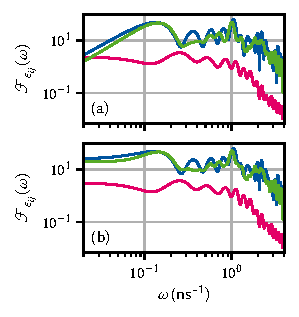
\includegraphics{img/pdf/filter_functions/CNOT_FF_unitary_v_complete}
    \caption[\imgsource{img/py/filter_functions/cnot_FF.py}]{
        Filter functions of the voltage detunings $\epsilon_{ij}$ excluding (a) and including (b) the zero-padded identity matrix basis element $C_0^c\propto\text{diag}(1,1,1,1,0,0)$ for the computational subspace.
        Evidently, including $C_0^c$ removes the \gls{dcg} character, namely that $F_{\epsilon_{ij}}(\omega)\rightarrow 0$ as $\omega\rightarrow 0$, of the gates but has little effect on the high-frequency behavior.
        As the pulse optimization minimizes, among other figures of merit, the infidelity of the final propagator mapped to the closest unitary on the computational subspace due to quasistatic and fast white noise, this indicates that excluding $C_0^c$ from the filter function corresponds to partially neglecting non-unitary components of the propagator on the computational subspace.
    }
    \label{fig:app:ff:filter_function:cnot}
\end{marginfigure}

Similar to the fidelity, we also obtain the canonical filter function shown in panel (b) of \cref{fig:ff:CNOT} by summing only over columns one through 15 of the control matrix, $F_{\epsilon_{ij}}(\omega) = \sum_{k=1}^{15}\bigl\lvert\ctrlmat_{\epsilon_{ij} k}(\omega)\bigr\rvert^2$.
In fact, including the first column, corresponding to the padded identity matrix $C_0^c$, in the filter function removes the \gls{dcg} character of $F_{\epsilon_{12}}(\omega)$ and $F_{\epsilon_{34}}(\omega)$, which instead approach a constant level of around 20 (note that the filter function is dimensionless in our units) at zero frequency.
This is consistent with the fact that the gates were optimized using quasistatic and fast white noise contributions to the fidelity after mapping to the closest unitary on the computational subspace.
We have performed Monte Carlo resimulations that support this reading.
In \cref{fig:app:ff:filter_function:cnot} we show the filter functions once including and once excluding the contributions from $C_0^c$.

% ==================================================
%           QFT GATES SECTION
% ==================================================
\subsection{\texorpdfstring{\acrshort{grape}}{GRAPE}-optimized gate set and validation of \texorpdfstring{\acrshort{qft}}{QFT} fidelities}\label{subsec:app:ff:fidelity:qft}
\begin{figure}
    \centering
    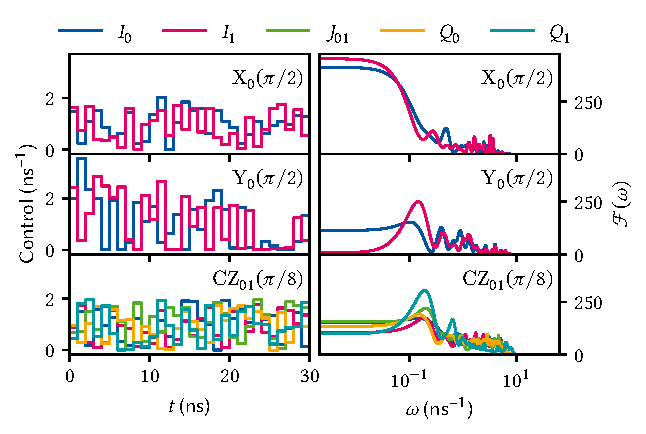
\includegraphics{img/pdf/filter_functions/qft_atomic_pulses}
    \caption[\imgsource{img/py/filter_functions/quantum_fourier_transform.py}]{
        Control fields (top row) and corresponding filter functions (bottom row) of the \acrshort{grape}-optimized pulses in $\mathbb{G}$.
        (a),(b) $\mr{X}_0(\pi/2)$; (c),(d) $\mr{Y}_0(\pi/2)$; (e),(f) $\mr{CR}_{01}(\pi/2^3)$.
        Note that the optimization is neither very sophisticated nor realistic as the algorithm only maximizes the systematic (coherent) fidelity $\mr{tr}\bigl(UQ\adjoint_\mr{targ}\bigr)/d$ and the randomly distributed initial control amplitudes are not subject to any constraints.
    }
    \label{fig:app:ff:qft:gates}
\end{figure}

In this section we give details on the \acrshort{grape}-optimized pulses for the gate set $\mathbb{G} = \lbrace\mr{X}_{i}(\pi/2),\mr{Y}_{i}(\pi/2),\mr{CR}_{ij}(\pi/2^3)\rbrace$ used in \cref{sec:ff:examples:qft} to simulate a \gls{qft} algorithm, and validate the fidelities using time-domain simulations.
As mentioned in the main text, we consider a toy Rabi driving model with \acrshort{iq} single-qubit control and exchange to mediate inter-qubit coupling.
Cast in the language of quantum optimal control theory this translates to a vanishing drift (static) Hamiltonian, $H_\mr{d} =  0$, and a control Hamiltonian in the rotating frame given by
\begin{gather}
    \Hc(t) = \Hc\gth{0}(t)\otimes\eye + \eye\otimes\Hc\gth{1}(t) + \Hc\gth{01}(t), \\
    \Hc\gth{i}(t) = I_i(t)\sx\gth{i} + Q_i(t)\sy\gth{i}, \\
    \Hc\gth{ij}(t) = J_{ij}(t)\sz\gth{i}\otimes\sz\gth{j},
\end{gather}
where $I_i(t)$ and $Q_i(t)$ are the in-phase and quadrature pulse envelopes and $\sigma_{x,y}\gth{i}$ are the Pauli matrices acting on the $i$th and extended trivially to the other qubit.
For simplicity, we assume periodic boundary conditions so that qubits 1 and 4 are nearest neighbors as well.
As our goal is only of illustrative nature and not to provide a detailed gate optimization, we obtain the controls $\lbrace I_0(t), Q_0(t), I_1(t), Q_1(t), J_{12}(t)\rbrace$ for the gate set $\mathbb{G}$ using the \acrshort{grape} algorithm implemented in \qutip~\cite{Johansson2012} initialized with randomly distributed amplitudes.
The resulting pulses and the corresponding filter functions for the relevant noise operators are shown in \cref{fig:app:ff:qft:gates}.

We now perform \gls{gksl} master equation and \gls{mc} simulations using the methods laid out in \cref{subsec:app:ff:time_domain_methods:methods} to verify the fidelities predicted for the \gls{qft} circuit in \cref{sec:ff:examples:qft}.
We focus on noise exclusively on the third qubit, entering through the noise operator $B_\alpha\equiv\sigma_y\gth{3}$.
We assemble the \gls{qft} circuit discussed in the main text from the gate set $\mathbb{G}$, obtaining the control Hamiltonian
\begin{equation}\label{eq:app:ff:control_hamiltonian:qft}
    \Hc(t) = \sum_{\langle i,j\rangle} I_i(t)\sx\gth{i} + Q_i(t)\sy\gth{i} + J_{ij}(t)\sz\gth{i}\otimes\sz\gth{j}.
\end{equation}
Similarly, we define the noise Hamiltonian as
\begin{equation}\label{eq:app:ff:noise_hamiltonian:qft}
    \Hn(t) = \sum_{\langle i,j\rangle} b_{I}(t)\sx\gth{i} + b_{Q}(t)\sy\gth{i} + b_{J}(t)\sz\gth{i}\otimes\sz\gth{j}
\end{equation}
with the noise fields $b_{\alpha}(t)$ for $\alpha\in\{I,Q,J\}$.
For the \gls{gksl} master equation, we set $L_\alpha\equiv\sigma_y\gth{3}$ as well as $\gamma_\alpha\equiv\flatfrac{S_0}{2}$ with $S_0$ the amplitude of the one-sided noise \gls{psd} so that $S(\omega) = S_0$.
For the \gls{mc} simulation, we explicitly generate time traces of $b_Q(t)$ (\cf \cref{eq:app:ff:noise_hamiltonian:qft}).
We choose an oversampling factor of 16 so that the time discretization of the simulation is $\Delta t_\mr{MC} = \flatfrac{\Delta t}{16} = \qty{62.5}{\pico\second}$ ($\Delta t = \qty{1}{\nano\second}$ is the time step of the pulses used in the \gls{ff} simulation), leading to a highest resolvable frequency of $\fmax = \qty{16}{\giga\hertz}$.
Conversely, we increase the frequency resolution by sampling a time trace longer by a given factor, giving frequencies below \fmin (\qty{16}{\kilo\hertz} for pink, \qty{0}{\hertz} for white noise) weight zero, and truncating it to the number of time steps in the algorithm times the oversampling factor.
This yields a time trace with frequencies $f\in [\fmin, \fmax]$ and a given resolution (we choose $\df = \qty{160}{\hertz}$).
For reference, we show the fidelity filter functions for the circuit with and without echo pulses in this frequency band in \cref{fig:app:qft_ff}.

\begin{figure}
    \centering
    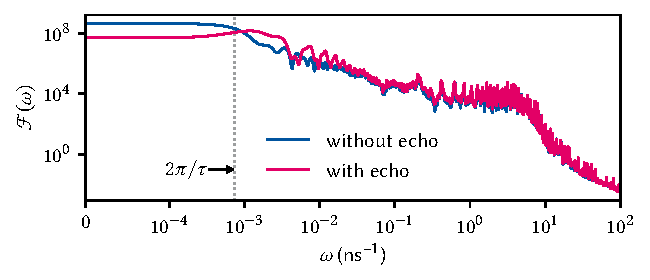
\includegraphics{img/pdf/filter_functions/qft_filter_function_Y3}
    \caption[\imgsource{img/py/filter_functions/quantum_fourier_transform.py}]{
        Filter functions for noise operator $\sigma_y\gth{3}$ for the \gls{qft} circuit without (blue) and with (magenta) additional echo pulses.
        Introducing the echoes shifts spectral weight towards higher frequencies, reducing the DC level of the filter function by two orders of magnitude and thus leading to an improved fidelity for \oneoverf noise.
    }
    \label{fig:app:qft_ff}
\end{figure}
\begin{table*}
    \centering
    \renewcommand\arraystretch{1.25}
    \caption{
        Infidelities $\avginfid = 1-\avgfid$ of the \gls{qft} circuit due to noise on $\sigma_y\gth{3}$.
        \Gls{mc} values are averages over $N=1000$ random traces and have a relative error of \qty{3}{\percent}.
        We included frequencies in the range of $\omega\in [0, 100]\,\unit{\per\nano\second}$ for white noise, and $\omega\in [\qty{100}{\per\milli\second}, \qty{100}{\per\nano\second}]$ for pink noise.
        \Gls{ff} values are computed with $n_\omega=1000$ samples logarithmically distributed over the same interval.
        Prefactors in the power law $S(\omega)= A\omega^\alpha$ are \qty{2e-6}{\per\nano\second} and \qty{1e-9}{\per\nano\second\squared}, respectively.
    }
    \label{tab:app:fidelities}
    % This table is automatically generated by img/py/filter_functions/qft_monte_carlo.py 
 \begin{tabular}{l *{4}{S[table-format=1.2e+1,round-mode=figures,round-precision=3]}}
\toprule
 & \multicolumn{2}{c}{\textsc{White noise}} & \multicolumn{2}{c}{\oneoverf \textsc{noise}} \\
\cmidrule(lr){2-3}\cmidrule(lr){4-5}
\textsc{Method} & \textsc{Without echo} & \textsc{With echo} & \textsc{Without echo} & \textsc{With echo} \\
\midrule
\acrshort{gksl} & 8.380261e-03 & 8.380835e-03 & {---} & {---} \\
\acrshort{mc} & 8.727031e-03 & 7.986534e-03 & 2.093929e-02 & 4.272077e-03 \\
\acrshort{ff} & 8.377560e-03 & 8.403532e-03 & 2.115425e-02 & 4.459941e-03 \\
\bottomrule
\end{tabular}

\end{table*}

\Cref{tab:app:fidelities} compares the infidelities $\infid=1-\fid$ from \gls{gksl} and \gls{mc} simulations to the filter function predictions following \cref{eq:ff:infidelity:ent}.
Note that the precise value of the filter function result depends quite sensitively on the frequency sampling due to the sharp peaks in the gigahertz range (\cref{fig:app:qft_ff}).
As the table shows, both the \gls{gksl} and the \gls{mc} calculations agree well with the predictions made by our filter-function formalism.

